Di seguito è riportato un diagramma che illustra le classi principali per la comunicazione tra Model-View-Controller.

\begin{figure}[H]
  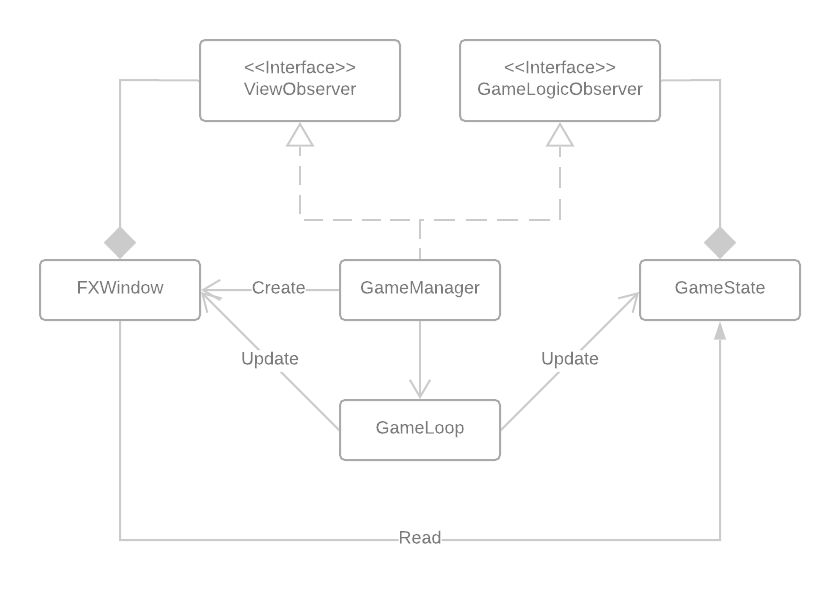
\includegraphics[width=15cm]{res/MVC_Diagram.png}
  \caption{Architettura}
\end{figure}

\subsection{MVC Pattern}
Per lo sviluppo del gioco si è scelto di utilizzare il pattern MVC in quanto si vuole avere una separazione pulita tra la parte logica e la parte di visualizzazione. In questo modo si lascia aperta la possibilità di avere diversi tipi di interfaccia grafica.

\subsubsection{Model} Contiene la logica di gioco. 

\subsubsection{View} Ha il compito di mostrare i dati forniti dal Model. Sarà costituita da due parti: il menù di gioco e l'arena di gioco.

\subsubsection{Controller} Fa da ponte tra Model e View, cattura gli eventi generati dalla view utilizzando il pattern Observer. Si occupa della lettura da file e della gestione dell'Event-Loop.

\subsection{Event-Loop}
Si è scelto di utilizzare un event-loop per gestire la ricezione di input utente, l'update della parte logica e l'update della parte di interfaccia grafica. 
Si è scelto di utilizzare un approccio ad event-loop single-thread, poiché, si adatta bene al tipo di gioco sviluppato. Inoltre l'approccio a event-loop, essendo in esecuzione su un singolo thread e processando un task alla volta, risulta essere thread safe, esulando da problemi implementativi in cui si poteva incorrere.


